\documentclass[tikz,border=10pt]{standalone}
\usepackage{tikz}
\usetikzlibrary{shapes.geometric, arrows.meta, positioning, fit, backgrounds, calc}

\begin{document}
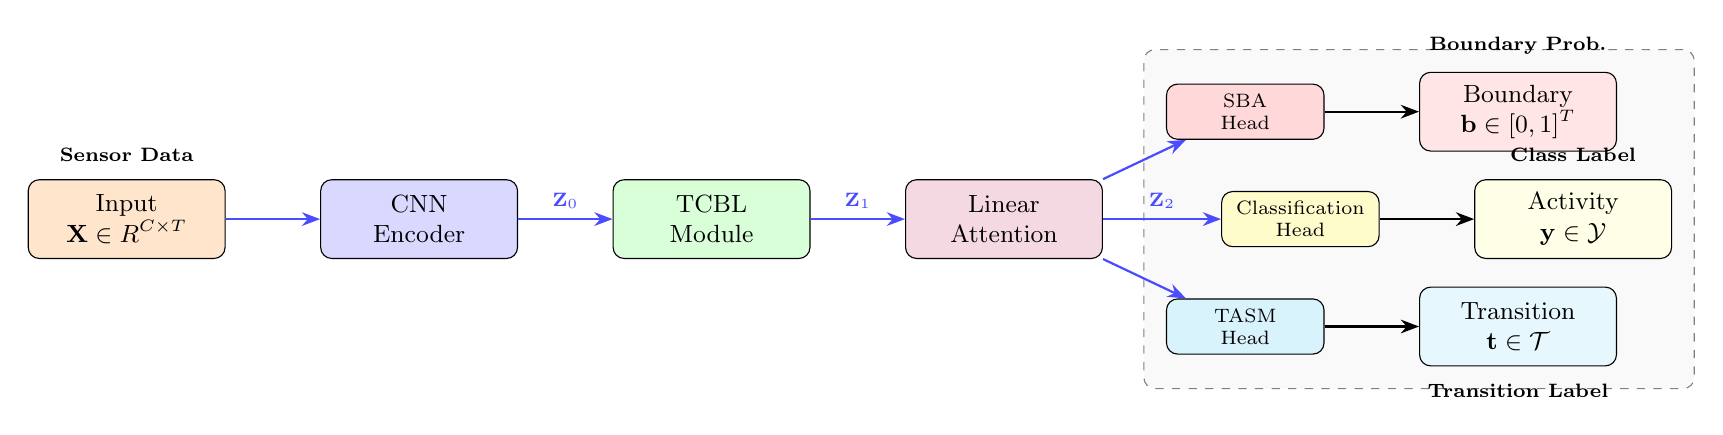
\begin{tikzpicture}[
    node distance=0.8cm and 1.2cm,
    block/.style={rectangle, draw, fill=blue!10, rounded corners, 
        minimum height=1cm, minimum width=2.5cm, align=center, font=\small},
    smallblock/.style={rectangle, draw, fill=green!10, rounded corners,
        minimum height=0.7cm, minimum width=2cm, align=center, font=\scriptsize},
    arrow/.style={-Stealth, thick},
    dataarrow/.style={-Stealth, thick, blue!70},
    label/.style={font=\scriptsize\bfseries}
]

% Input
\node[block, fill=orange!20] (input) {Input\\$\mathbf{X} \in \mathbb{R}^{C \times T}$};

% CNN Encoder
\node[block, fill=blue!15, right=of input] (cnn) {CNN\\Encoder};

% TCBL Module
\node[block, fill=green!15, right=of cnn] (tcbl) {TCBL\\Module};

% Transformer Encoder
\node[block, fill=purple!15, right=of tcbl] (trans) {Linear\\Attention};

% Split into three heads
\node[smallblock, fill=red!15, above right=0.5cm and 0.8cm of trans] (sba) {SBA\\Head};
\node[smallblock, fill=yellow!20, right=1.5cm of trans] (cls) {Classification\\Head};
\node[smallblock, fill=cyan!15, below right=0.5cm and 0.8cm of trans] (tasm) {TASM\\Head};

% Outputs
\node[block, fill=red!10, right=of sba] (bound) {Boundary\\$\mathbf{b} \in [0,1]^T$};
\node[block, fill=yellow!10, right=of cls] (activity) {Activity\\$\mathbf{y} \in \mathcal{Y}$};
\node[block, fill=cyan!10, right=of tasm] (transout) {Transition\\$\mathbf{t} \in \mathcal{T}$};

% Arrows
\draw[dataarrow] (input) -- (cnn);
\draw[dataarrow] (cnn) -- node[above, font=\scriptsize] {$\mathbf{Z}_0$} (tcbl);
\draw[dataarrow] (tcbl) -- node[above, font=\scriptsize] {$\mathbf{Z}_1$} (trans);
\draw[dataarrow] (trans) -- node[above, font=\scriptsize] {$\mathbf{Z}_2$} (cls);
\draw[dataarrow] (trans.north east) -- (sba);
\draw[dataarrow] (trans.south east) -- (tasm);
\draw[arrow] (sba) -- (bound);
\draw[arrow] (cls) -- (activity);
\draw[arrow] (tasm) -- (transout);

% Labels
\node[label, above=0.1cm of input] {Sensor Data};
\node[label, above=0.1cm of bound] {Boundary Prob.};
\node[label, above=0.1cm of activity] {Class Label};
\node[label, below=0.1cm of transout] {Transition Label};

% Background for multi-task learning
\begin{scope}[on background layer]
    \node[fit=(sba)(cls)(tasm)(bound)(activity)(transout), 
          draw=gray, dashed, rounded corners, 
          fill=gray!5, inner sep=8pt,
          label={[font=\scriptsize\itshape]above:Multi-Task Learning}] {};
\end{scope}

\end{tikzpicture}
\end{document}
